documentclass[border=5mm]{standalone}
\usepackage{amsmath}
\usepackage{pgfplots}
\usetikzlibrary{plotmarks}
\pgfplotsset{compat=newest}
\begin{document}
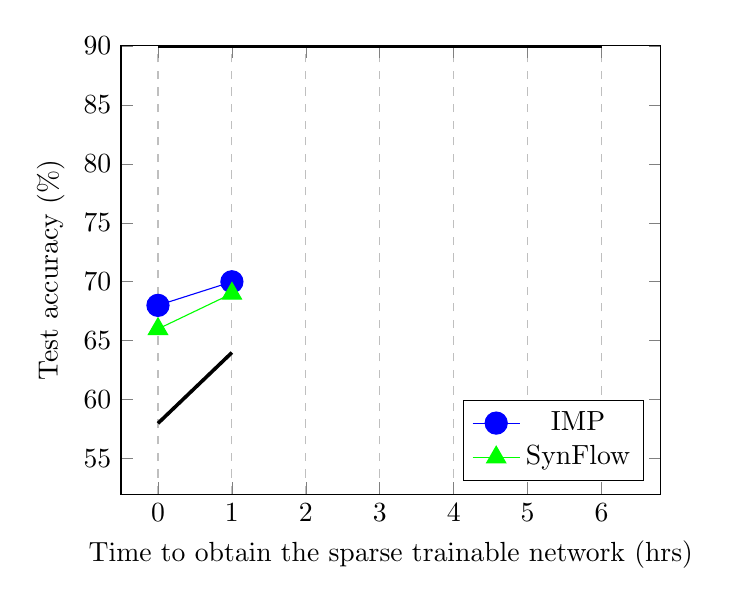
\begin{tikzpicture}
    \begin{axis}[
        xlabel={Time to obtain the sparse trainable network (hrs)},
        ylabel={Test accuracy (\%)},
        xmin=-0.5,xmax=6.8,
        ymin=52,ymax=90,
        xtick={0,1,...,7},
        ytick={55,60,65,...,90},
        xmajorgrids=true,
        grid style=dashed,
        legend pos=south east,
        mark size=4,
        cycle list={
            {blue,mark=*},
            {green,mark=triangle*},
            {black,line width=1.3pt,forget plot}
        },
        legend entries={IMP,SynFlow,SNIP,Unpruned Accuracy},
        ]
        \addplot coordinates {(0,68) (1,70)};
        \addplot coordinates {(0,66) (1,69)};
        \addplot coordinates {(0,58) (1,64)};
        \addplot coordinates {(0,90) (1,90) (2,90) (3,90) (4,90) (5,90) (6,90)};
    \end{axis}
\end{tikzpicture}
\end{document}